\newif\ifdraft
\drafttrue
%\draftfalse

\ifdraft
  \documentclass[draft]{llncs}
  \usepackage{color}
  \usepackage[normalem]{ulem}
  \definecolor{green}{rgb}{.2,.8,0}
  \definecolor{blue}{rgb}{0,0,1}
  \definecolor{red}{rgb}{1,0,0}

  \usepackage[final]{graphicx}  
  
  \newcommand{\change}[1]{\textcolor{green}{#1}}
  \newcommand{\delete}[1]{\textcolor{red}{\sout{#1}}}
  \newcommand{\tbc}[1]{\textcolor{blue}{#1}}
  \newcommand{\todo}[1]{\textbf{\color{red}{TO-DO}}: #1}
  \newcommand{\mnote}[1]{\marginnote{#1}}
  
\else
  \documentclass{llncs}
  \usepackage{graphicx}
  
  \newcommand{\change}[1]{#1}
  \newcommand{\delete}[1]{}
  \newcommand{\tbc}[1]{#1}
  \newcommand{\todo}[1]{}
  \newcommand{\mnote}[1]{}
\fi

\usepackage{url}
\usepackage{alltt,verbatim}
\usepackage{soul}
\usepackage{subfig}
\usepackage{pifont}
\usepackage[utf8]{inputenc}

\usepackage[all]{xy}
\newcommand{\code}[1]{{\texttt{#1}}}

% MARGIN NOTES
\marginparwidth 1.25 true in

\newcounter{marginalnote}
\setcounter{marginalnote}{1}
\renewcommand{\themarginalnote}{\roman{marginalnote}}
\newcommand{\marginnote}[1]
           {\raisebox{1ex}{\scriptsize (\themarginalnote)}%
            \marginpar{\footnotesize\raggedright\indent
                       \raisebox{1ex}{\scriptsize (\themarginalnote)} #1}%
            \addtocounter{marginalnote}{1}}
% MARGIN NOTES

% Maude code
\usepackage[final]{listings}
\usepackage{xcolor}
\lstdefinelanguage{maude}
{
	alsoletter={\:},
    morecomment=[l]{---},
    morecomment=[l]{***},
    keywords={pr, protecting, sort, sorts, subsort, subsorts, including, class, msg, msgs, endfm, fmod, is, mod, endm, omod, endom},
    keywords=[2]{eq,  mb, ceq, if, rl, crl, else, then, fi},
    keywords=[3]{ctor, assoc, comm, gather, id\:},
    keywords=[4]{op, ops, var, vars}
}

\lstset{
  language=maude,
  basicstyle=\ttfamily\footnotesize,
  frame=tb,
	framerule=0.2pt,
  %keywordstyle=\bfseries,
	%keywordstyle=[2]\bfseries,
	%keywordstyle=[3]\bfseries,
	%keywordstyle=[4]\bfseries,
}
% Maude code

\DeclareGraphicsExtensions{.png}

\begin{document}

\pagestyle{headings} % switches on printing of running heads
%\addtocmark{XXXX} % additional mark in the TOC

\title{Solving The Movie Database Case: A solution using the Maude-based e-Motions tool}
\titlerunning{TO-DO} % abbreviated title (for running head) also used for the TOC unless \toctitle is used

\author{Antonio~Moreno-Delgado \and Francisco~Dur\'an}
\authorrunning{Moreno et al.} %abbreviated author list (for running head)

%%%% modified list of authors for the TOC (add the affiliations)
\tocauthor{
  Antonio Moreno-Delgado (Universidad de M\'alaga),
  Francisco Dur\'an (Universidad de M\'alaga)
}

\institute{
    University of M\'alaga\\
    \email{\{amoreno,duran\}@lcc.uma.es}
    }

\maketitle

\begin{abstract}

\end{abstract}

%-------------------------------------------------------------
%  INTRODUCTION
%-------------------------------------------------------------
\section{Introduction}\label{sec:intro}

\todo{two sentences introducing Maude}

Maude may be seen as a general framework where to develop model transformations. In this way, some work has been done~\cite{TroyaV10}. Since a term is very general, one could specify graphs or models as terms. Thus, a Maude module can define a \textit{in-place} model transformation, where rewriting rules define transitions between two states or models.

e-Motions~\cite{RiveraDV10} is a Domain-Specific Modeling Language (DSML) and a very general tool that supports the specification and simulation of any real-time DSML. Artifacts developed in e-Motions are translated to Maude in a transparent way. The e-Motions simulation is achieved using the Maude engine. Therefore, e-Motions can be seen as a framework where graphically code in Maude.

\subsection{e-Motions}\label{sub:emotions}
For the sake of comprehension of the rest of the paper, in this section we briefly present e-Motions. The definition of a Domain-Specific Language (DSL) typically comprises three tasks: (i) the definition of its abstract syntax, (ii) the definition of its concrete syntax and (iii) the specification of its behavior.

In e-Motions the abstract syntax is defined by means of a Ecore metamodel, in which all the language concepts and the relations between them are specified. The concrete syntax is provided by defining the so-called Graphical Concrete Syntax (GCS). A GCS is a model (conforms the GCS metamodel) where an image is attached to each concept defined in the abstract syntax.

In e-Motions the behavior of a DSL is specified using visual graph-transformation rules. An e-Motions rule consists of a---possibly conditional---Left-Hand Side (LHS), a Right-Hand Side (RHS) and zero or more Negative Application Conditions (NACs). The LHS defines a (sub)-graph matching, optionally conditional. The RHS specifies a (sub)-graph replacement, which if the rule is applied, every object in the LHS that is not in the RHS is deleted, new objects in the RHS that are not in the LHS are created, and those objects whose attributes (or links) are changed are updated. NACs specify conditions or (sub)-graphs such that if there is a matching, the rule cannot be fired.

Fig.~\ref{fig:assemble} shows an example of an e-Motions rule.\footnote{System documentation and several examples are available at \url{http://atenea.lcc.uma.es/e-Motions}.} The objects in both the RHS and LHS are represented by their images defined in the GCS model. Rule \code{Assemble}'s LHS defines the precondition of the rule. It models a assemble machine who needs both a head and a handle in its connected conveyor. If the \code{NAC1}, stating that the current matched \code{Assemble} has not unfinished other rule, is not satisfied, the rule can be applied. The rule is applied as follows. All objects in the LHS which they do not appear in the RHS are deleted, i.e. \code{he} and \code{ha} objects. Those objects in the RHS which do not appear in the LHS are created, setting their attributes properly, i.e. the \code{ham} object with its three attributes. The rest of objects remain changeless. Moreover, as e-Motions is a framework where to define real-time systems, each rule is applied in a established time, i.e. \code{[prodTime,prodTime]} in the \code{Assemble} rule. A rule may contain zero or more local or auxiliary variables. All attribute or variable assignments and conditions are expressed using Object-Constraint Language (OCL)~\cite{ocl}.

The abstract and concrete syntax, and the behavior of a DSL are models and the e-Motions tool has been developed following MDE principles. The Maude code corresponding to a system defined in e-Motions is generated by an ATL/TCS transformation~\cite{atl}.

\begin{figure}[htp]
  \centering
  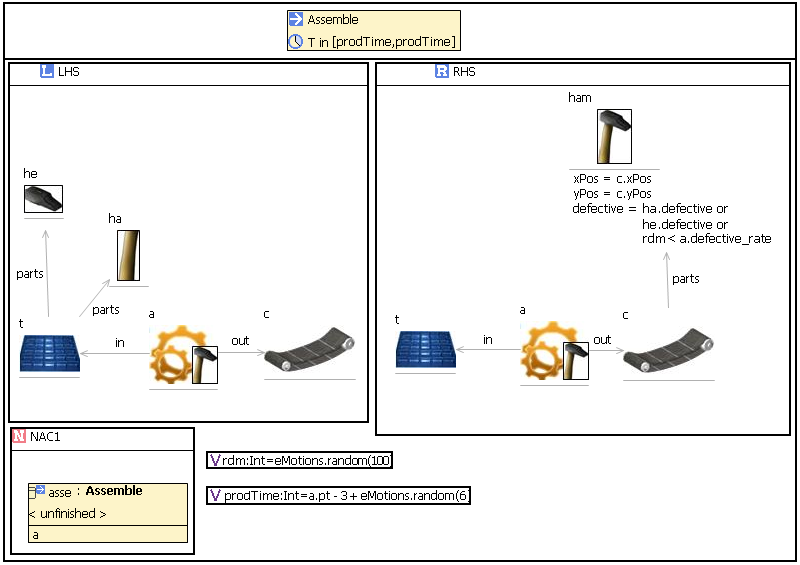
\includegraphics[width=\textwidth]{imgs/assemble}
  \caption{e-Motions \code{Assemble} rule.}\label{fig:assemble}
\end{figure}

%-------------------------------------------------------------
% SOLUTIONS
%-------------------------------------------------------------
\section{Solution}\label{sec:solution}

\delete{Since e-Motions supports in a very intuitive, user-close and visual way, we show how the IMDb problem~\cite{imdbcase} can be solved using it. Each task is solved using the definition of a DSL, which shares in general the abstract and concrete syntax. The rewrite rules defining the behavior depends on the solution given. All rewrite rules are \textit{instantaneous}, since the case to be solved do not have time requirements.}

We show how the IMDb problem can be solved using e-Motions tool. Each task is figured out using the definition of a DSL, which shares, in general, the abstract and concrete syntax. In fact, the abstract syntax is given in advance in~\cite{imdbsources}. The rewrite rules defining the behavior depends on the concrete task and its solution. All rewrite rules are \textit{instantaneous}, since the case to be solved do not have time requirements.

e-Motions is very general: it supports OCL expressions and time requirements. This makes that the Maude code generated by e-Motions tool is not as time performant as desired. Together with the e-Motions solution we present a optimized Maude solution for each task. 


\todo{terminar esta sección:}

e-Motions-based solution which are visual, very intuitive and very close to the problem domain are shown against Maude-based solution. Although Maude-based solutions are also very expressive, the fact that  

Both e-Motions-based and Maude-based solutions are very expressive and very close to the problem domain

Finally, although e-Motions is presented as a Eclipse tool, we run the simulations with the code generated by it directly in a Maude instance, since the transformation from a e-Motions-based system into Maude code takes time.

\subsection{Task 1}\label{sub:task1}

Task 1 comprises the generation of synthetic models (conforming the movie database metamodel~\cite{imdbcase}) from an input parameter $N \geq 0$. In the following we present an e-Motions based solution and a Maude solution. 


\subsubsection{e-Motions-based solution.}

Following an e-Motions based approach, we define the abstract and concrete syntax and the behavior of our so-called \textit{Task 1 DSL}. Taking a parameter $N$ as input model, \textit{Task 1 DSL} generates a model containing synthetic data.

As it has been introduced in Section~\ref{sub:emotions}, the abstract syntax of a DSL is given in e-Motions by means of a Ecore metamodel. In fact, this metamodel is provided beforehand in~\cite{imdbsources}. We call this metamodel \textit{Movies MM}. However, the \textit{parameter N} has to be modeled in some way, since in e-Motions the state is just a model. Hence, a new concept call \code{Parameter} has been added to Movies MM. This results in a so-called \textit{Movies* MM}. The class \code{Parameter} has two integer attributes \code{nP} and \code{nN}, positive graphs and negative graphs, due to data generation following Henshing graphs~\cite{henshing} is divided into positive and negative cases.

For the concrete syntax, Fig.~\ref{fig:concreteSyntax} shows how an image has been attached to each concept modeled in the Movies* MM. The behavior of this \textit{Task 1 DSL} is given by means of two in-place rules: \code{createPositive} and \code{createNegative}. Figure~\ref{fig:createPositive} shows the \code{createPositive} rule, which takes an object \code{p} of type \textit{Parameter} with \textit{nP} attribute greater or equal than $0$ and, after the rule application, synthetic data conforming to the Henshin rules~\cite{henshing} are created. Fig.~\ref{fig:createNegative} shows the \code{createNegative} rule, which is analogously defined.

Once the syntax and the behavior of the system has been coded, the user may specify a model, which conforms to \textit{Movies* MM}, containing an object \code{Parameter} with its two attributes \code{nP} and \code{nN} properly set. This model is used as initial model of the execution.

This solution is really close to the problem specification~\cite{imdbcase}. Both Fig.~\ref{fig:task1} and Fig.~2 in~\cite{imdbcase} specifying the data generation are almost the same. This solution demonstrates how close is the solution to the problem domain, and how user-friendly is e-Motions.

\subsubsection{Maude version.}
This proposal of Task 1 consists of a object-based Maude specification, which is composed by two main modules: the \code{MOVIES@MM} module defining the classes structure and the \code{TASK1} module defining the solution. The solution is coded using again two rules: \code{createPositive} and \code{createNegative}. One could realized that the Maude version is very much like the e-Motions version. In fact, the former is almost the textual version of the latter. Listing~\ref{lst:createPositive} shows the \code{createPositive} Maude rule that takes the \code{createPositive(N:Nat)} message and a \code{freshOid} auxiliary message---used to create new object identifiers---and returns such a object configuration conforming the Henshin specification~\cite{imdbcase}.

The messages \code{createPositive} and \code{createNegative} are generated in zero-rewrite steps with the equation showed in Listing~\ref{lst:createexampleeq}.

\begin{lstlisting}[caption=\code{createPositive} Maude rule., label=lst:createPositive]
rl [createPositive] :
  createPositive(N)
  freshOid(N')
=>
  < N'     : Movie | rating : (10.0 * float(N)) >
  < N' + 1 : Movie | rating : (10.0 * float(N) + 1.0) >
  < N' + 2 : Movie | rating : (10.0 * float(N) + 2.0) >
  < N' + 3 : Movie | rating : (10.0 * float(N) + 3.0) >
  < N' + 4 : Movie | rating : (10.0 * float(N) + 4.0) >
  
  < N' + 5 : Actor | name : ("a" + string((10 * N),     10)),
                   movies : (N', N' + 1, N' + 2, N' + 3)     >
  < N' + 6 : Actor | name : ("a" + string((10 * N + 1), 10)),
                   movies : (N', N' + 1, N' + 2)             >
  < N' + 7 : Actor | name : ("a" + string((10 * N + 2), 10)),
                   movies : (N' + 1, N' + 2, N' + 3)         >
  < N' + 8 : Actress | name : ("a" + string((10 * N + 3), 10)),
                   movies : (N' + 1, N' + 2, N' + 3, N' + 4) >
  < N' + 9 : Actress | name : ("a" + string((10 * N + 4), 10)),
                   movies : (N' + 1, N' + 2, N' + 3, N' + 4) >
  freshOid(N' + 10) .
\end{lstlisting}

\begin{lstlisting}[label=lst:createexampleeq, caption=Equation \code{createExample(N:Nat)}.]
eq createExample(0) = none .
eq createExample(s(N)) = createPositive(N)
                         createNegative(N)
                         createExample(N) .
\end{lstlisting}


\begin{figure}[htp]
  \subfloat[Actor.\label{fig:actor}]{
    \makebox[60px][c]{
\includegraphics[scale=1]{imgs/actor}}
  }
  \hfill
  \subfloat[Actress.\label{fig:actress}]{
    \makebox[60px][c]{
\includegraphics[scale=1]{imgs/actress}}
  }
  \hfill
  \subfloat[Movie.\label{fig:movie}]{
    \makebox[60px][c]{
\includegraphics[scale=1]{imgs/movie}}
  }
  \hfill
  \subfloat[Couple.\label{fig:couple}]{
    \makebox[60px][c]{
\includegraphics[scale=1]{imgs/couple}}
  }
  \hfill
  \subfloat[Parameter.\label{fig:parameter}]{
    \makebox[60px][c]{
\includegraphics[scale=1]{imgs/parameter}}
  }
  \caption{Concrete syntax for \textit{Movies* MM}.}
  \label{fig:concreteSyntax}
\end{figure}

\todo{Correctness?}

\todo{Tiempos}

\begin{figure}[htp]
  \subfloat[The \code{createPositive} rule.\label{fig:createPositive}]{%
    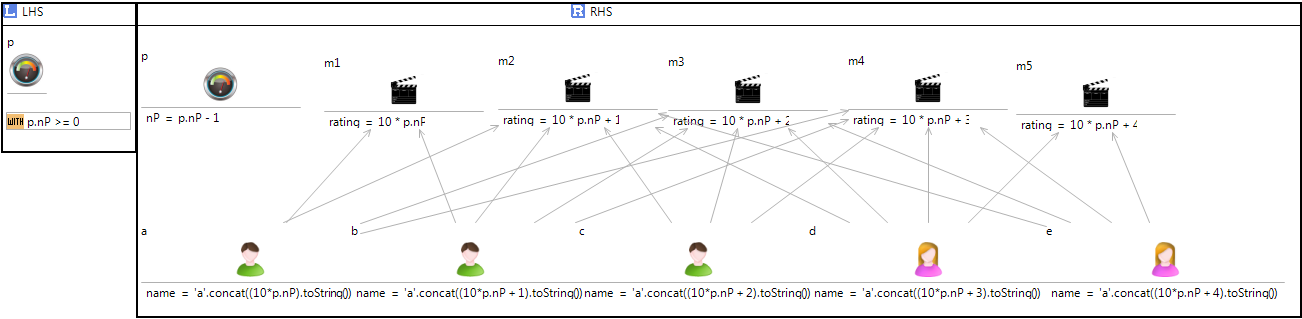
\includegraphics[width=\textheight, angle=90]{imgs/createPositiveRule}
  }
  \hfill
%  \subfloat[Rules' headers.]{
%    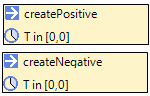
\includegraphics[width=0.2\textwidth]{imgs/headersCreate}
%  }
%  \hfill
  \subfloat[The \code{negativePositive} rule.\label{fig:createNegative}]{%
    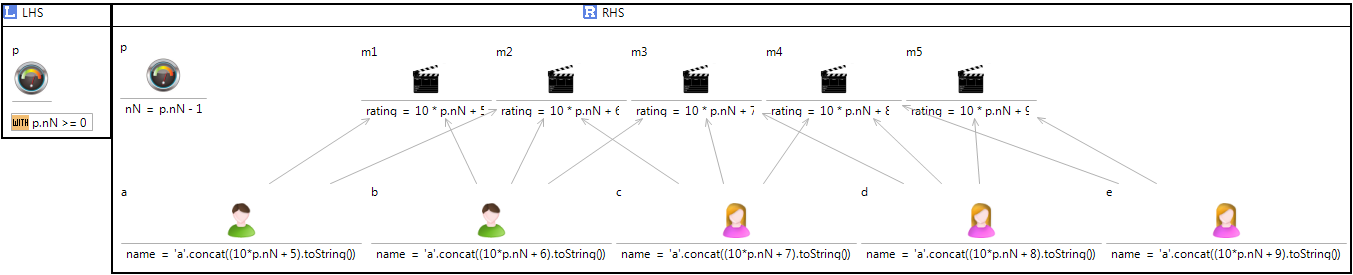
\includegraphics[width=\textheight, angle=90]{imgs/createNegativeRule}
  }
 
  \caption{Task 1 rules. \label{fig:task1}}
\end{figure}

\subsection{Task 2}
Task 2 consists of extract all couples from a given model, either from Task 1 or IMBd database~\cite{imdbsources}. Two persons are couple whether they played together in at least three movies~\cite{imdbcase}. Once again we present the e-Motions and the Maude solution.

\subsubsection{e-Motions-based solution}

Fig.~\ref{fig:createCouple} shows the \code{createCouple} rule which implements the whole task. \code{Person} objects are shown using square shapes because \code{Person} is an abstract class and it does not have image attached. The \code{createCouple} rule consists of a LHS with a OCL condition, which states \textit{``LHS holds iff there are two persons \code{per1} and \code{per2}, such that the number of movies in the intersection between \code{per1}'s movies and \code{per2}'s movies is greater or equal than 3''}. Moreover, the \code{coupleHasNotBeenCreated} NAC avoids the application of the rule if the couple already exists. 

However, although this solution works, one can notice that the number of matchings in the LHS of the rule is combinatorial. The fact that there are such a large number of matchings makes this solution too inefficient. \todo{add numbers supporting this.}

\begin{figure}[htp]
  \centering
  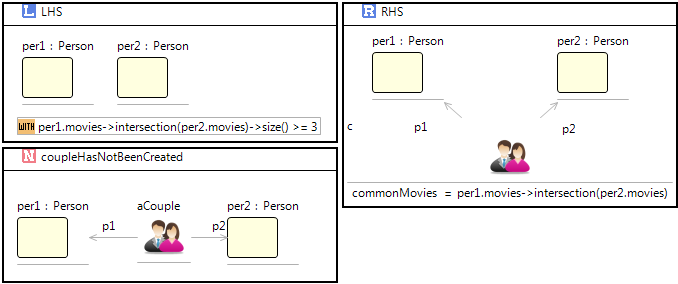
\includegraphics[width=\textwidth]{imgs/ruleCouples}
  \caption{\code{createCouple} rule.}\label{fig:createCouple}
\end{figure}

We have implemented another solution in which we limit the number of matchings using the next algorithm:
\begin{enumerate}
  \item We split \code{Person}s and \code{Movie}s into separate configurations.
  \item We fix a \code{Person}.
  \item Given a \code{Person}, we look for all couples.
  \item Whether the current \code{Person} set has been gone over all the other persons, we set the next person, and the current person is move to the resulting collection.
\end{enumerate}

Following this approach the number of persons to match as possible couple decrease. A new concept so-called \code{Collection} is added to the metamodel with its concrete syntax to implement the algorithm above mentioned. Fig.~\ref{fig:areCouples} shows one of the rules specified for this solution,\footnote{The rest of the rules are available at \url{https://github.com/antmordel/ttc14emotions}.} namely those that creates new couples. The box is the concrete syntax for the \code{Collection} concept.

\begin{figure}[htp]
  \centering
  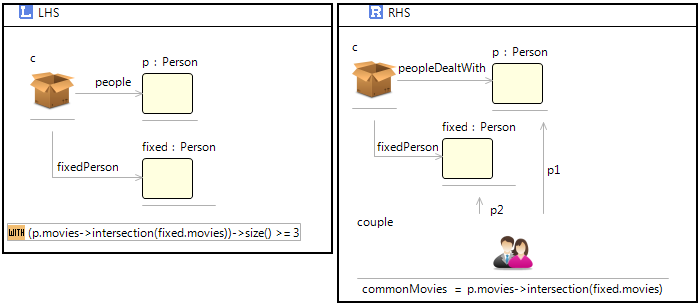
\includegraphics[width=\textwidth]{imgs/areCouples}
  \caption{\code{doingCouples} rule.}\label{fig:areCouples}
\end{figure}

\todo{add numbers}

\subsubsection{Maude-based solution}


\section{Conclusions}

\bibliographystyle{splncs03}
\bibliography{TTC14}
\providecommand{\url}[1]{\texttt{#1}}
\end{document}
